% Created 2022-03-22 Tue 23:57
% Intended LaTeX compiler: pdflatex
\documentclass[11pt]{article}
\usepackage[utf8]{inputenc}
\usepackage[T1]{fontenc}
\usepackage{graphicx}
\usepackage{longtable}
\usepackage{wrapfig}
\usepackage{rotating}
\usepackage[normalem]{ulem}
\usepackage{amsmath}
\usepackage{amssymb}
\usepackage{capt-of}
\usepackage{hyperref}
\usepackage{gensymb}
\usepackage{circuitikz}
\usepackage{tikz}
\usepackage{minted}
\usepackage[margin=2cm]{geometry}
\usepackage{fancyhdr}
\pagestyle{fancy}
\fancyhf{}
\fancyhead[L]{{\textcolor{gray}\leftmark}}
\fancyhead[R]{{\textcolor{gray}\thepage}}
\renewcommand{\headrulewidth}{0pt}
\usepackage{url}
\usepackage{rotfloat}
\usepackage{tikz}
\usepackage{float}
\hypersetup{hidelinks}
\usepackage{gensymb}
\usepackage{amsmath}
\numberwithin{equation}{section}
\usepackage{chngcntr}
\counterwithin{figure}{section}
\counterwithin{table}{section}
\usepackage{amssymb}
\newcommand {\R}{\mathbb{R}}
\usepackage{gensymb}
\usepackage{booktabs}
\usepackage{minted}[linenos]
\usepackage{sourcecodepro}
\definecolor{deepblue}{rgb}{0.0, 0.18, 0.39}
\setlength{\parindent}{0}
\usepackage{parskip}
\usepackage{enumitem}
\setlist{noitemsep}
\usepackage[format=plain, labelfont={bf}, textfont=it]{caption}
\usepackage{booktabs}
\usepackage[framemethod=tikz]{mdframed}
\BeforeBeginEnvironment{minted}{\begin{mdframed}[style=sourcecode]}
\AfterEndEnvironment{minted}{\end{mdframed}}
\date{\today}
\title{Floating Island - ISDP Group 33}
\hypersetup{
 pdfauthor={Ben Frazer},
 pdftitle={Floating Island - ISDP Group 33},
 pdfkeywords={},
 pdfsubject={},
 pdfcreator={Emacs 27.2 (Org mode 9.6)}, 
 pdflang={English}}
\begin{document}

\maketitle
\mdfdefinestyle{sourcecode}{%
%backgroundcolor=darkgray,
skipabove=12pt,
hidealllines=true,
apptotikzsetting={%
  \tikzset{mdfbackground/.append style={fill=deepblue,fill opacity=0.1}}},
leftline=true,%innerleftmargin=10,innerrightmargin=10,
innerleftmargin=25,
linewidth = 4pt,
roundcorner = 2pt,
linecolor= darkgray,
%#frametitlerule=true,frametitlerulecolor=green,
%#frametitlebackgroundcolor=darkgray,
%#frametitlerulewidth=2pt
}
\begin{table}[H]
\caption{Authors}
\centering
\begin{tabular}{lll}
\toprule
Last Name & Forename & Student number\\
\midrule
Ameh & Ilebo Naomi & 2655446A\\
Bai & Jingwei & 2698327B\\
Deng & Binbin & 2631250D\\
Frazer & Benjamin & 2704250F\\
Gao & Baorong & 2637530G\\
Hu & Yike & 2748951H\\
Huo & Kairun & 2674596H\\
Shiyamsunthar & Partheepan & 2531525S\\
Xiao & Yao & 2630063X\\
Zhu & Xu & 2669120Z\\
\bottomrule
\end{tabular}
\end{table}

\tableofcontents

\section{Executive Summary}
\label{sec:org55c18df}
As governments, scientists and communities deploy strategies to mitigate and reverse the effects of climate change, proposals to adapt to the predicted changes to the planet are also pursued. The use of more renewable energy, increasing energy efficiency of devices and carbon sequestration are aimed at mitigating some proven causes of climate change. This report however deals with adapting to one of the noted effects of climate change- rising sea levels.

Global sea level rise forecast for the year \texttt{2100} range between \texttt{0.6-1.1m}. Coastal communities will gradually lose habitable land as sea levels rise due to warming. As the sea encroaches into communities, beaches, and hospitality establishments, this will displace people and businesses and affect economies dependent on waterfront hospitality businesses. To tackle this problem, the concept of floating villages has been earmarked as a potential solution.

In certain parts of the world, people have lived in houseboats and floating houses but usually at docks. For this project, the village is set up a few miles out to sea. The aim of the project is to create a design that will serve as a test bed for technologies that may be deployed for floating villages in the future. While there are many challenges to be tackled to create a community offshore, this report focuses on a select few. Upon successful deployment of the solutions proffered in this prototype, they may be scaled up to tackle the displacement of people caused by rising sea levels.

The specific areas covered by the report are structural/architectural, energy supply, connection to the mainland as well as environmental and economic sustainability. An overview of each section is presented below:

\subsection{Platform Design and Architecture}
\label{sec:org15bb6a2}
Platform floatation is devised by using eco-friendly concrete to reinforce the exterior of the platform while being hollow in the middle to trap air allowing the platform to float via the buoyancy criteria and will house structures composed of reinforced wood. The platform will be moored to the ocean floor via bio-rock and will have anti-roll stabilisation technologies incorporated.

\subsection{Environmental Sustainability}
\label{sec:org483f527}
The environmental sustainability section covers the water supply and waste management solutions. It also projects the possible environmental impact of other aspects of the project. The final decision is to establish a connection to the water and sewage systems on the mainland for stability and cost reasons. All decisions made for the projects ideally ensure low environmental impact and indicators to monitor are itemised

\subsection{Communication and Physical connection}
\label{sec:org0951e43}
5G base stations will be established around the floating village. Due to the short transmission distance of 5G, a ship will be added in the transmission process, which is used to strengthen signal amplification called USV.  For the physical connection between the floating village and mainland, a floating dock will be built using the pontoon construction technique. This method provides an easy and flexible way to satisfy the physical connection for both workers and visitors. For the details of the floating dock, the material has been chosen as 6061-T1 aluminium alloy rather than conventional steel because aluminium alloy has more appropriate physical properties and cheaper total cost.

\subsection{Energy Supply}
\label{sec:orge06f6ca}
Offshore wind power as the main power generation method, combining diesel generators to ensure stable energy supply in the event of an emergency or in the absence of high wind for a period of time. Additionally, it is useful to install rechargeable batteries in case of an emergency and the best way is to use Li-ion batteries because of its low self-discharge rate.

The solutions proffered provide effective methods to solve the challenges, but they are also chosen to minimise the impact to the sea flora and fauna, use clean/renewable technology where possible to avoid unintended outcomes. In general, the solutions proffered are important steps towards creating an adaptation strategy for rising sea levels.

\subsection{Cost}
\label{sec:org7bfe10c}
The project is assumed to attract an investment of about \texttt{7} million. A construction and annual maintenance cost estimate was completed based on estimates made from research of existing systems. Using the payback formula, it is calculated that it would take \texttt{7.89} years to complete recoup the investment. Finally, the sources of revenue for the hotel are presented and some strategies are given to increase the revenue of the hotel, such as creating brand value/personality, marketing, etc., to accelerate the rate of return.

\section{Introduction}
\label{sec:orgbcc646c}
The most potent crisis faced by humanity is arguably the impact of climate change on the world and its lasting effects on our lives. Climate change has battered us in numerous ways such as forest fires, unprecedented floods, harsh droughts and rapidly increasing sea levels. These are some of the common examples, but humanity must persevere amongst the climate crises.

Losing land mass due to increasing sea levels is considered a critical issue since it directly correlates to lost homes and livelihoods and there are no known ways to prevent the rise of sea level. Therefore, if we lose the dependence on solid land and move human settlements to the open sea, we can offset the negative impacts of rising sea levels.

To combat the rise of sea level, as a team, we have devised a plan to emulate a small village that is modelled to be a tourist attraction to fund itself through its operation. The village will be constructed to withstand the sea environment, capable of handling and delivering power, contains modern communication facilities and is environmentally friendly.


\section{Platform Design and Architecture}
\label{sec:orgb79f7fb}
\subsection{Background}
\label{sec:orge9418ae}
The focus of this project is a community set in the open sea, relatively distant from the nearest land mass. The structural mass supporting the community needs to be safe from natural phenomena and resistant to environmental wear and tear while being sustainable and environment friendly.

\subsection{Structure Design}
\label{sec:org23e4839}
\subsubsection{Platform}
\label{sec:orgaa7d887}
As the basic part of the building, the selection of platform materials is very important. The platform not only serves as the support of the superstructure, but is also an important structure to ensure the overall stability of the building.

This requires that the main body of the platform must be rigid, but cannot sink. Using a material that can float easily (like wood) is not suitable as a deck material. Wood is relatively weather resistant and rigid to maintain a lot of mass on top of it but long term exposure to seawater immersion will greatly shorten the service life of wood- which is unacceptable for aquatic buildings. In addition, considering the concept of green sustainable development, this study does not consider the use of materials that are extremely harmful to the marine ecosystem, such as plastic bottles or plastic materials.

Using common building materials such as concrete and steel will achieve our ultimate goal, but these materials alone cannot withstand the degradation caused by seawater, so we will turn our view towards a composite concrete mix created by the Kleindienst Group, which promotes coral growth regarding its structure \cite{1s}. To achieve a rigid floating platform, we can choose to trap air within the concrete-wrapped structure as shown in Figure \ref{platform_img}, such that the large amount of trapped air will cause the structure to float. Using this method, we don't rely entirely on the material's ability to float, but rather the material provides rigidity and the trapped air provides buoyancy to keep the platform afloat.

Moreover, this concrete base can be prefabricated on land to complete the required size, and then transported to the required location for assembly, which avoids the disadvantages that the concrete is not easy to consolidate and the strength is easily reduced in a humid and low-temperature environment. The size of the platform will determine the weight the superstructure can carry. The greater the weight, the greater the air space reserved in the concrete block to increase the buoyancy required.

\begin{figure}[H]
\centering
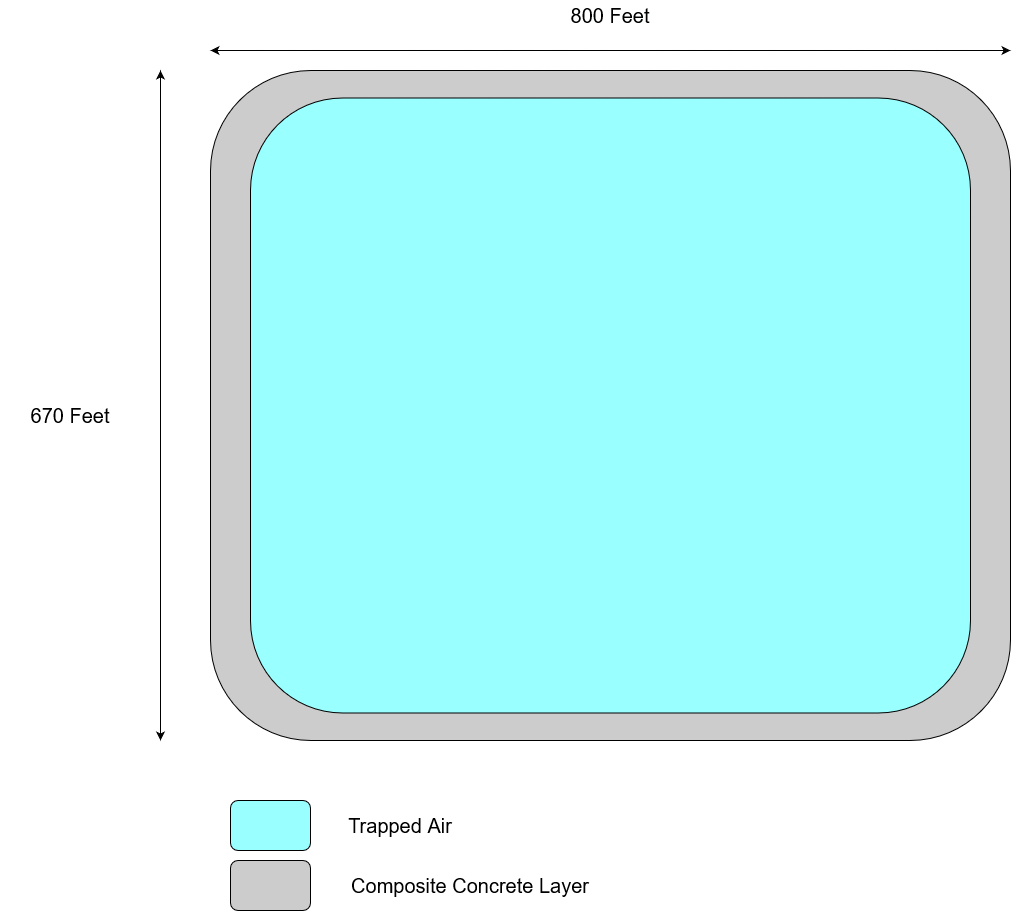
\includegraphics[width=0.8\textwidth]{Figures/platform_img.png}
\caption{\label{platform_img}Bird’s eye cross sectional view of the platform.}
\end{figure}


\subsubsection{Main Building}
\label{sec:org96fec14}
In modern buildings, reinforced concrete, steel structure and wood structure are the three mainstream structures, and these three materials are also applicable in this project. Table \ref{Structural_MaterialScoringTable} is the detailed scoring results for determining the best material selection in this project \footnote{All criteria are scored 0-10}.

\begin{table}[H]
\caption{\label{Structural_MaterialScoringTable}Scoring of structure}
\centering
\begin{tabular}{lrrr}
\toprule
Structure & Wood & Steel & Concrete and steel\\
\midrule
Environmental Impact & 10 & 6 & 6\\
Energy Consumption & 4 & 5 & 6\\
Maintainability & 4 & 5 & 6\\
Practicality & 10 & 10 & 8\\
Dynamic Nature & 8 & 8 & 4\\
Cost effectiveness & 5 & 3 & 4\\
\midrule
Total & 41 & 37 & 34\\
\bottomrule
\end{tabular}
\end{table}

\begin{itemize}
\item \textbf{Environmental Impact:} 0 is detrimental and 10 has no negative impacts.
\item \textbf{Energy Consumption:} 0 is a power-hungry option
\item \textbf{Maintainability:} 0 represents an option that requires constant attention and 10 is a option that's very easy to maintain
\item \textbf{Practicality:} 0 represents an option that is not practically proven to work while 10 represents an option that is easy to incorporate with many real world counterparts/examples.
\item \textbf{Dynamic Nature:} 0 is for a option that's not a smart and 10 represents a smart option
\item \textbf{Cost effectiveness:} 0 represents an expensive option and 10 represents a cheap option.
\end{itemize}

By comparison, the project uses wood structure as building material. From the perspective of environmental protection, it is a renewable material, and as a building material, it has the least impact on the environment from production to waste. Earthquake-resistant wooden structure villa has good life safety performance in the event of an earthquake and the same in the water for the vibration of the waves, but also has good absorption performance.

For wooden houses, the wooden beams and the wooden columns can be connected by tenon joints. This method of fixing the two pieces of materials together by the friction of the materials can make the whole structure combine quite firmly. The main structure is staggered through tenon joints to improve stability. The design of the wooden structure house follows the law of design force, adopts the beam-column structure system, uses the beam-column structure with large span as the main force transmission system, transfers the vertical and horizontal loads to the platform through the beam-column, and at the same time a large number of components with small cross-sections are evenly and densely linked, and the structural skeleton works with wall panels, floor panels and roof panels to carry various loads at the same time, and then transmit this force to the platform. The two structures are designed to bear the load and ensure the stability of the structure.

\subsection{Mooring}
\label{sec:orgd952f2e}
As an aquatic structure, the method used to keep the building stationary on the water is a critical issue. Once our structure has been made to specification, the next hurdle is the concept of mooring the structure to avoid it drifting into the open sea. The platform may be moored via two methods, both of which are sustainable to the environment but one approach has little to no energy consumption which is a crucial factor to our project, as energy is a luxury commodity and the other proves to be capable of withstanding natural phenomena.

In the first method, a solid foundation is created using 40-foot-long hydraulic legs that can stabilise and even lift the platform out of the water allowing them to withstand high winds and hurricanes  \cite{4s}, as seen in Figure \ref{40_foot_structure}. These legs are to be made of reinforced waterproof steel with a sealed extendable beam inside which lifts the platform. This system uses hydraulic fluid which can be detrimental to the environment. The amount of energy used to operate the legs is significant, but it could be offset by using solar power though energy is still scarce in our scenario.

\begin{figure}[H]
\centering
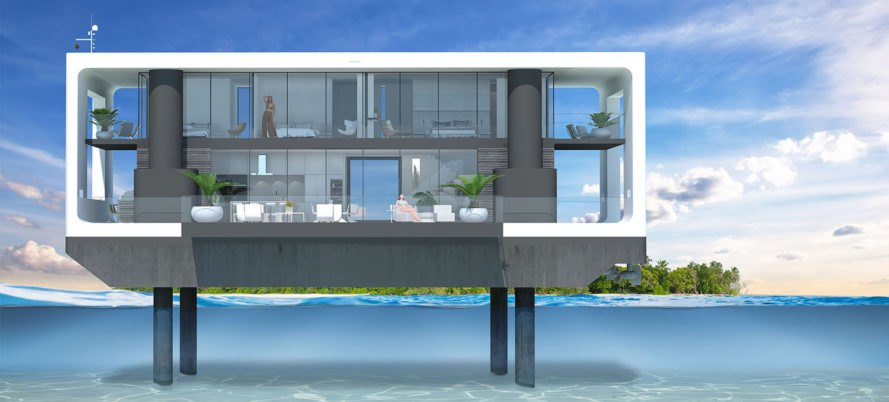
\includegraphics[width=0.8\textwidth]{Figures/40_foot_structure.jpg}
\caption{\label{40_foot_structure}Aquatic structure supported by hydraulic legs \cite{4s}}
\end{figure}

The second method uses Biorock as an anchor for our platform. Rust resistant steel cables will run from our platform to the seabed. Then, a small DC current will be passed through these cables to perform an electrolysis effect such that the salt from the sea water creates a solid limestone rock that affixes itself to the seabed, as seen in Figure \ref{bio_rock}. The Biorock will act as a strong anchorage point while boosting the growth of coral and flora in the ecosystem \cite{2s} which will further strengthen the hold onto the seabed.

\begin{figure}[H]
\centering
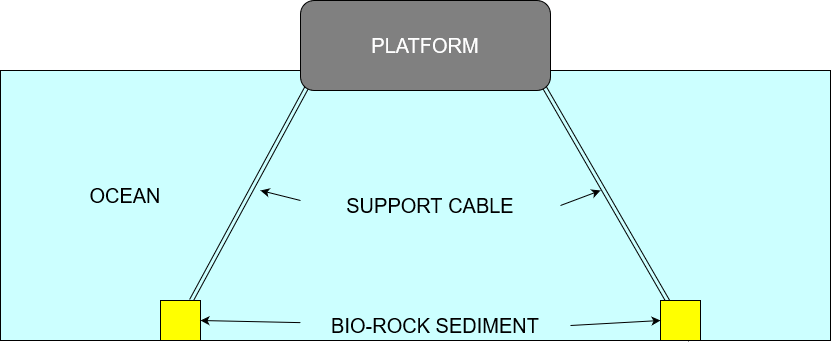
\includegraphics[width=0.8\textwidth]{Figures/bio_rock.png}
\caption{\label{bio_rock}Design implementation of BioRock mooring}
\end{figure}

It's clear that the hydraulic leg design is less favourable since the risk of hydraulic fluid leaking onto the ocean can be detrimental to the ocean ecosystem and there is an energy requirement to drive the hydraulic system. The Biorock approach is environmentally favourable and only requires energy during its initial setup, although it alone cannot face hurricanes and strong tidal waves. The use of hurricane proof floats can support the anchorage during heavy winds and the use of wave barriers, constructed using the same composite concrete used in the platform, to dampen \cite{10.1016/j.finel.2014.02.002} the waves around the village can help mitigate dangers to the inhabitants using the Biorock anchor method.

\subsection{Stabilisation}
\label{sec:org4c78b18}
While having the platform float on the sea surface surrounded by wave barriers stops harsh waves from entering the village, smaller waves are bound to impact the platform which will cause constant rocking and discomfort to the inhabitants. To reduce the impact by the waves, the platform must be modified to add stabilising elements.

To dampen a platform, one option is to consider an approach similar to vehicle suspension systems which consists of magneto-rheological dampers. A suite of these dampeners would be held between two sets of platforms where the lower platform will be directly in contact with the waves while the upper platform will house the occupants and structures, as shown in Figure \ref{mag_rheo}. When the waves impinge on the lower platform the force of the impact is absorbed by the dampeners, which contain fluids that can be influenced via electromagnetism, to avoid the force being transferred to the upper platform. The dampeners will be controlled by a control system that will determine how the fluids react to different wave impact forces.

\begin{figure}[H]
\centering
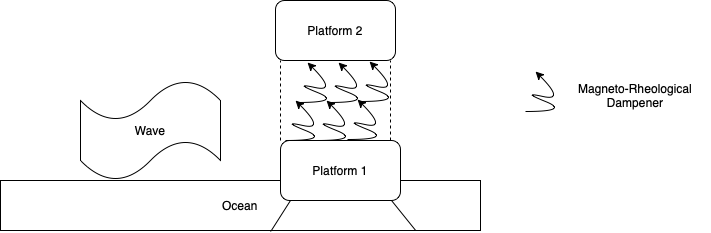
\includegraphics[width=0.8\textwidth]{Figures/mag_rheo.png}
\caption{\label{mag_rheo}Cross sectional view of dampening system}
\end{figure}

The second option considered is an anti-roll U – tank system which is a U shaped tank filled with water to a specific level to a specific level to stabilise a structure, as shown in Figure \ref{u_tank}. The structure is attached at the middle of the platform and will extend out towards the corners of the platform but will not interfere with the mooring of the platform. These systems have control valves built-in to transfer water across both ends of the tanks to retain the desired water level so that a structure can remain undisturbed. When waves are experienced by the platform, it would cause the platform to tilt and the control system attached to the tank will determine how much water needs to be transferred to prevent the platform from tilting thus stabilising the platform \cite{5s,6s}. The system is equipped with level sensors to determine the current water level and it will be part of the control system used to transfer water between both tanks.

\begin{figure}[H]
\centering
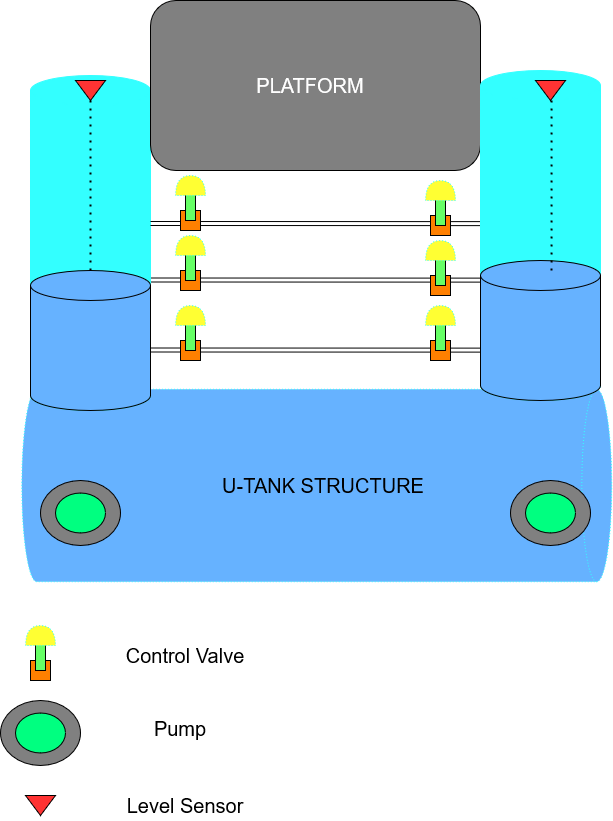
\includegraphics[width=0.8\textwidth]{Figures/u_tank.png}
\caption{\label{u_tank}U - Tank Anti Roll Design Implementation}
\end{figure}

When the two methods are analysed, it is clear that the magneto-rheological damping system carries high environmental impact since a small leakage of fluid will cause severe damage to the ecosystem. It is also not a maintenance friendly system as failure would result in having to take apart two separate platforms- increasing down time and increasing the cost associated with the lost time. Lastly, the cost associated with converting a system used by automobiles for stabilisation on the sea is very high since the concept has not been practically proven to work, thus research into the method will need to be needed.

The U-Tank system, however, is a proven technology \cite{6s} commonly used in most vessels for active stabilisation and the system is considerably maintenance friendly as it is a standalone structure upon which the platform resides- thus it can be removed from the platform to be worked on while a temporary system takes its place. The system does have wear and tear- it can shed some materials to the ocean. Therefore, there is a cost associated with remodelling the existing technology to be more environmentally friendly.

Even though both technologies prove to be semi-autonomous the ideal choice for this application is the U-tank system to reduce the impact of the waves.

\subsection{Village Layout}
\label{sec:orgf2f35c3}
Following the design and stabilisation aspect of the floating platform, the orientation of the platforms is considered next. The goal is to create a hotel that accommodates guests and provides comfort to the guests while being a practical solution for living on the open sea. Orientation can be in the form of a single platform that houses the hotel building or one main building with sub platforms that act as rooms or points of interest for the guests.

Having one major platform will aid reduced construction costs and make it easier to stabilise and monitor the platform leading to less maintenance costs down the road. The cost associated with stabilisation will be drastically reduced since only one platform needs to be moored and dampened, however since the scale of the platform is large the cost will be greater but not greater than having multiples of the similar technology. From the point of view of the guest, a single platform which houses all the activities may not be desirable and some would prefer privacy with their own space.

Using a spider-net structure such that the main building is in the centre of the village with pathways routing to each building or room, as seen in Figure \ref{village_layout}, may attract more people to its unique structure and the use of branched platforms will help spread the effect of waves almost acting like a natural damping system where the impact of the waves are lost over time as they travel through each platform. However, the cost associated with this orientation is large since we have now introduced multiple platforms all introducing construction and stabilisation costs which leads to increased maintenance cost down the road.

\begin{figure}[H]
\centering
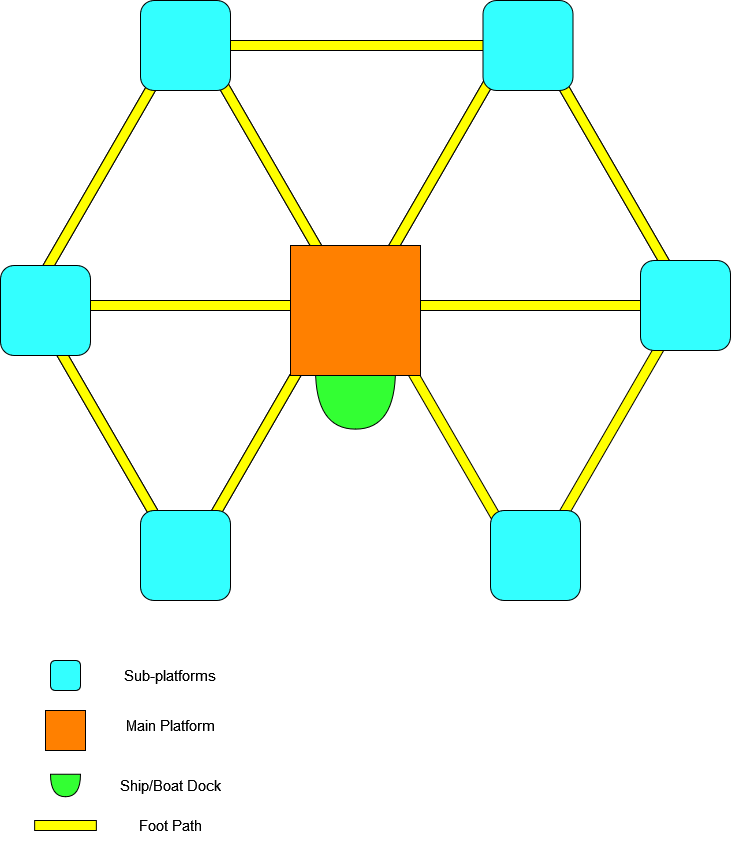
\includegraphics[width=0.8\textwidth]{Figures/village_layout.png}
\caption{\label{village_layout}Floating Village proposed layout}
\end{figure}

From a cost standpoint, the single platform orientation is an obvious choice, but this village is designed to attract guests and the village must be constructed in such a manner that would not bore the guests. Therefore, the choice to construct the village in a pattern where there are multiple smaller platforms connected to a larger hub would seem ideal. The cost associated with this orientation choice is undesirable, but it will be offset by the revenue brought in by the hotel.

\section{Power}
\label{sec:orge89416c}
As the floating village is isolated from the gas and electricity network on the mainland, it is necessary to provide access to energy for all the hotel staff and guests. The technical solutions and cost of power generation and storage are discussed in this section.

\subsection{Power generation}
\label{sec:orgbdec2d7}
To find the best way to generate power, a comparison was made between some primary power generation technologies (such as solar energy, wind energy, Tide energy, fossil fuel), where benefits and technical challenges were considered. Offshore wind power is chosen as the primary means of generating power for the following reasons:
\begin{enumerate}
\item Sea winds are much more frequent and powerful than land winds, which increases its availability.
\item Offshore wind power farms are far from human dwellings so they can be designed to maximise efficiency without worrying too much about noise pollution.
\item As they are all structures at sea, the power farms can serve more flexibly for floating villages.
\end{enumerate}

\subsubsection{Technical solutions}
\label{sec:orgb10f66c}
The principle of wind energy is the conversion of kinetic energy from wind into mechanical energy, which is then converted into electrical energy via a generator. The wind rotates the turbine blades, which turns the generator shaft that cuts through a magnetic field. And finally the energy accumulation device maintains a constant current output. Modern offshore wind turbines usually consist of wind turbine blades, low speed shaft, high speed shaft, anemometer, tower, generator, and hydraulic system. Among them, the blades convert wind energy into a machine that can change the direction of the wind turbine according to the change of wind direction, thus maximising the use of wind energy. The tower is a support to connect and support the wind turbine and generator, and its height depends on the surrounding terrain and the size of the wind turbine to ensure normal operation. A generator is a device that converts mechanical energy into electrical energy.
As for power transmission, we apply wireless transmission. Power farms aim at the floating villages and use laser beams to transfer power to them. This technique can transport energy long distances without obvious effect to human’s health. A power farm supplies electricity for several floating villages and the general layout is just like figure \ref{powerTransmission}.

\begin{figure}[H]
\centering
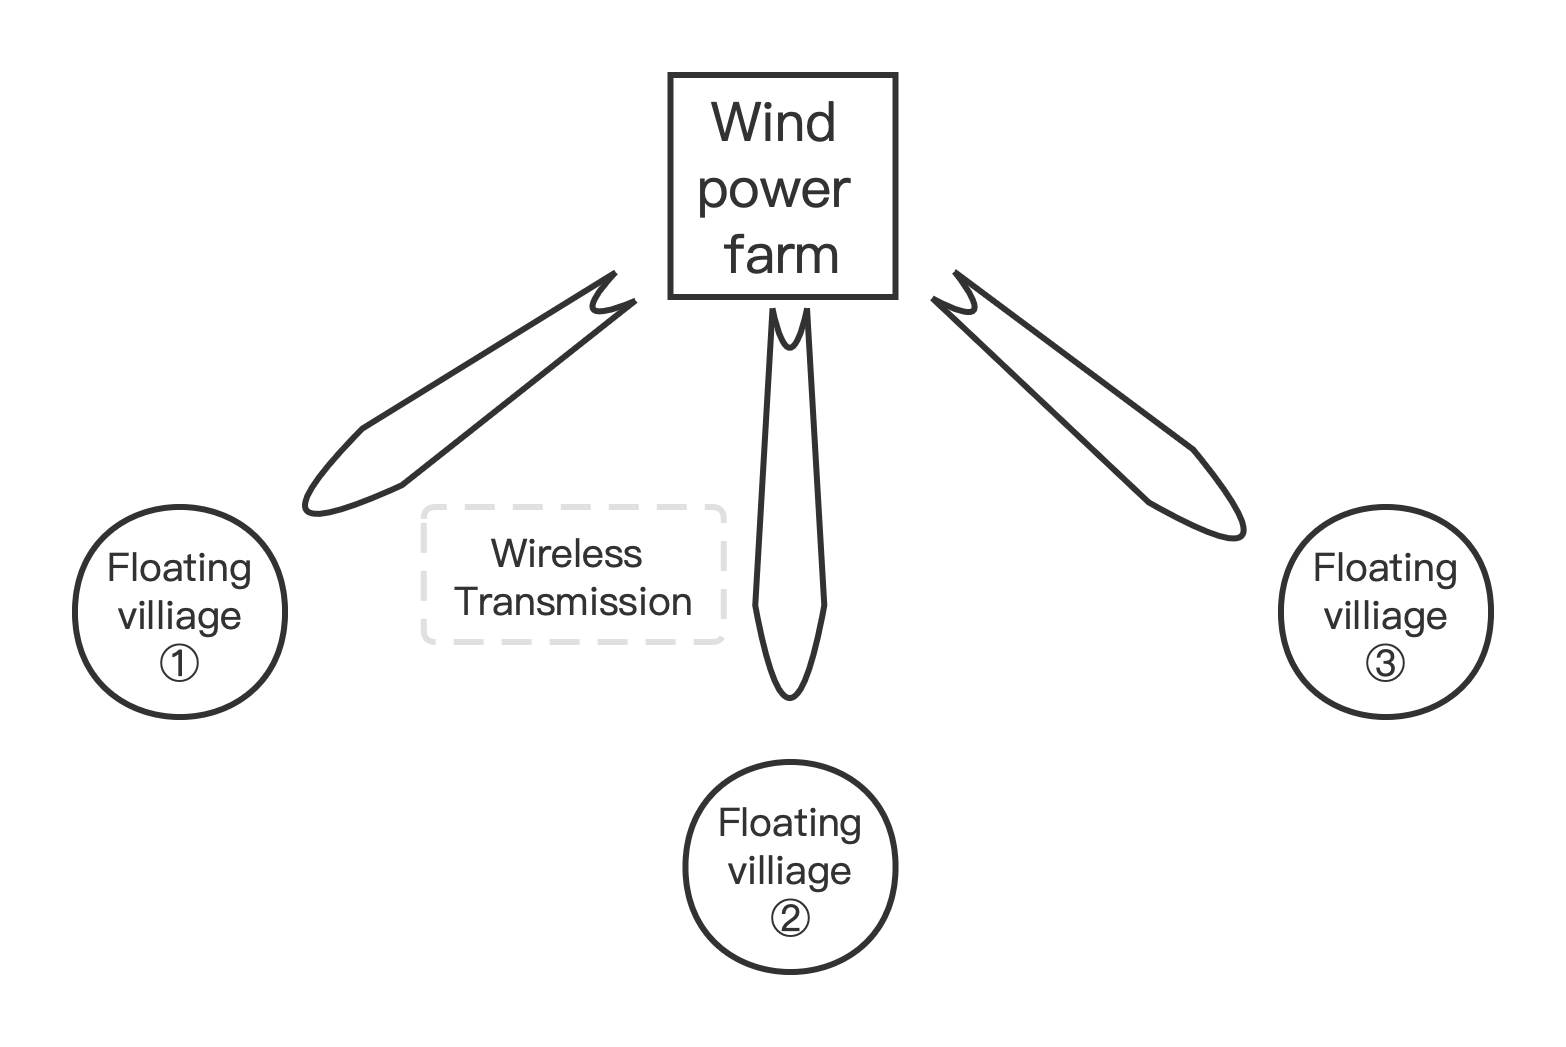
\includegraphics[width=0.8\textwidth]{Figures/powerTransmission.png}
\caption{\label{powerTransmission}Power transmission layout}
\end{figure}

\subsection{Cost breakdown}
\label{sec:org75a2940}
The total fixed cost for power generation equipment is about \texttt{£1,400,000}, including a \texttt{2 MW} wind turbine construction and installation fee. The operation and maintenance costs account for \texttt{1\%} of the total equipment costs, which is \texttt{£14,000}.

\begin{figure}[H]
\centering
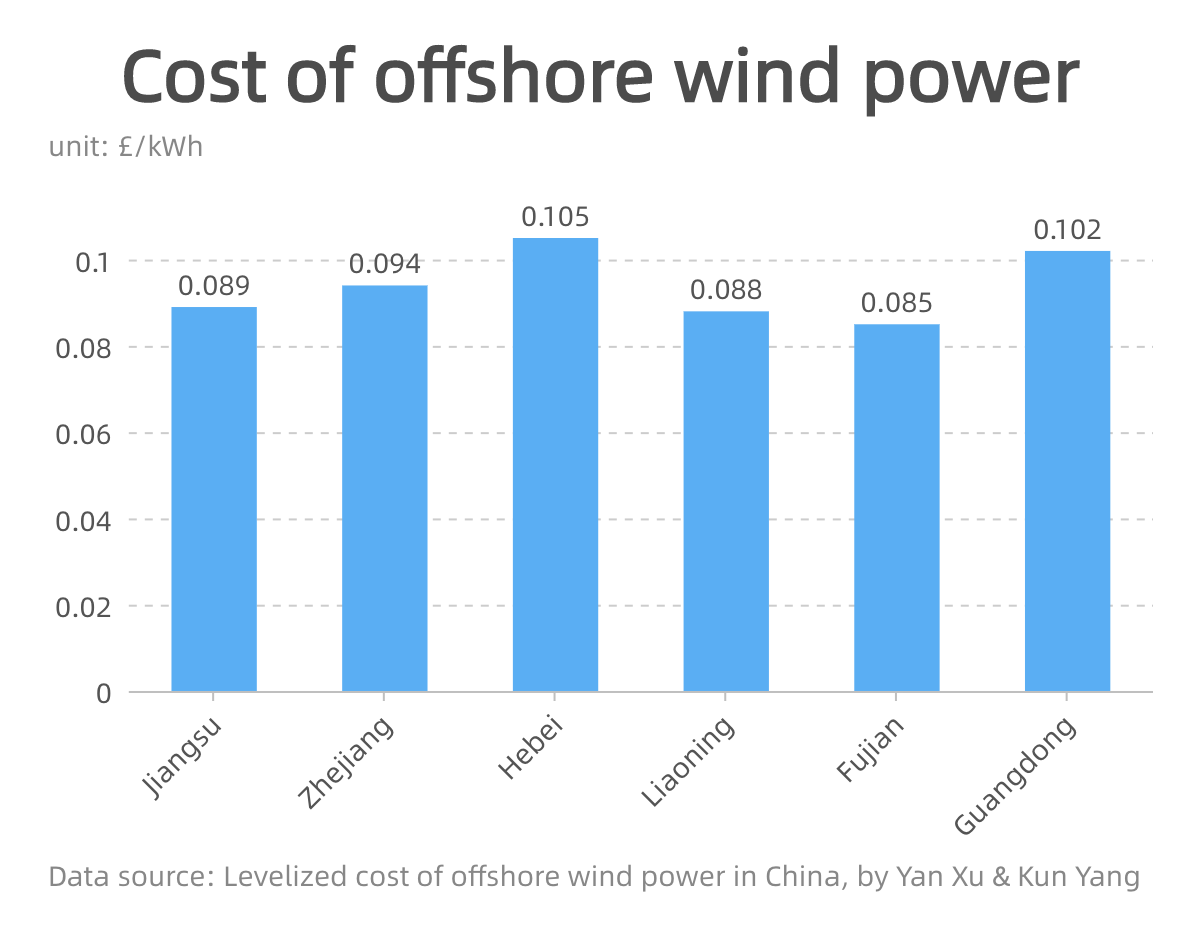
\includegraphics[width=0.8\textwidth]{Figures/powerGenerationCost.png}
\caption{\label{powerGenerationCost}Unit cost of offshore wind power in six typical provinces of China}
\end{figure}

As we can see in Figure \ref{powerGenerationCost}, the cost of offshore wind power generally ranges from \texttt{0.085 £/kWh} to \texttt{0.105 £/kWh} \cite{10.1016/j.ijepes.2021.107273}. Here, we set \texttt{0.09 £/kWh} as the unit cost. We assume that the resident population is \texttt{40} and each person consumes \texttt{4,500 kWh} electricity per year. It is necessary to generate an additional two months of electrical energy to store in case of temporary disability of power generating. Apart from the residents’ daily usage of electricity, floating villages’ basic operation activity, like mooring, stabilisation and so on, consumes \texttt{50,000 kWh} per year.   The yearly cost of generating power is:

\begin{align}
\label{eqEnergyCost}
\left[4,500kW\times 40\times \frac{14}{12}+ 50,000kWh\right]\times 0.09 \pounds /kWh = \pounds23,400/year.
\end{align}

In summary, the fixed cost of power generation  is \texttt{£1,400,000}, and the annual cost is \texttt{£37,400}.

\subsubsection{Energy Storage}
\label{sec:org077a248}
In case of an emergency, the absence of wind or very low speeds, it’s necessary to consider energy storage in this floating village. There are many kinds of energy storage technologies, each has its respective pros and cons. For example, lithium-ion batteries are very attractive because of their effective operation on a small scale. Also, they are lightweight and have good round-trip efficiency. But they require protection from being overcharged and completely discharged. On the contrary, the pumped hydro has a very large operation scale, good round-trip efficiency and the cost of each unit is very low. As for flywheels, they have low efficiency and can’t store a large amount of power, but they can transmit a large amount of power in a short time, which also helps to stabilise the frequency.

\subsubsection{Solutions}
\label{sec:org6f97276}
On wind farms it is necessary to use diesel generator systems as auxiliary to supply auxiliary loads, which is cost effective and fuel efficient. Additionally, rechargeable batteries will be used to store power because of the small scale and low prices.

According to the common characteristics of different chemical batteries below, the most suitable way for this project is to use Li-ion materials because of its low self-discharge rate. The cost of energy storage by Li-ion batteries per kWh can be hypothesised as around \texttt{£106} \cite{123}.

\begin{table}[H]
\caption{\label{CharacteristicsOfBatteries}Common characteristics of different chemical batteries}
\centering
\begin{tabular}{lll}
\toprule
Technology & Pros\xa0 & Cons\\
\midrule
NiMH & Cheap+ Larger capacity & High self-discharge rate\\
NiCd & Cheap & Memory effects + Toxic Cd  \footnotemark\\
NiZn & Cheap+ No toxic materials & High self-discharge rate\\
Li-ion & nan & Lower self-discharge rate\\
\bottomrule
\end{tabular}
\end{table}\footnotetext[2]{\label{orgbca6937}The battery memory effect is a reduction in the longevity of a rechargeable battery's charge, due to incomplete discharge in previous uses.}
\subsection{Storage Cost}
\label{sec:orgc6e3d76}
The lifetime cost of small-scale battery storage is now around \texttt{13 p/kWh} \cite{1234}. Storing 1 kWh of power generation every day for \texttt{300} days of the year is worth about \texttt{£40}. At the moment the cost per kWh of storage (all-in installed cost) is about \texttt{£400}, and so the payback time for a system is around \texttt{10} years.

Energy use per person in \texttt{2019} in United Kingdom is \texttt{4500 kWh} \cite{12345}, while the amount of energy use per day in the floating village is \(4500/365 \times 20 = 250 kWh\). In this situation, the capacity of the battery system is assumed to be \texttt{1500 kWh}, which is enough for \texttt{40} people to live on the island for \texttt{3} days.

An \texttt{80 kW} diesel generator costs \texttt{£15.000} \cite{123abc} and consumes diesel \texttt{24 litres/hr} \cite{123bcd}. The cost of diesel is around \texttt{150 p/litre} \cite{123cde} and it’s \texttt{£315,360} for the whole year. The final price of power storage in floating village is derived in Equation \ref{eqSomeCalc} \footnote{Includes one year consumption of diesel}:

\begin{align}
\label{eqSomeCalc}
1500\times\pounds106 + \pounds15,000 + \pounds315,360 = \pounds 490,000
\end{align}

\section{Communication and Transport}
\label{sec:orga7ab480}
\subsection{Communication technology}
\label{sec:orga7bd287}
Maritime communication technology is the most important means to ensure normal communication between the mainland and the village.  Satellite communication is widely used in maritime communication technology, but this method has the limitation of high delay and low transmission efficiency. The new fifth-generation communication technology can satisfy the demand for maritime broadband as shown in \ref{A_novel_platform_of_maritime_communication_network}.

\subsubsection{The Coast-5G-Based Network}
\label{sec:org44261b9}
With advantages like broadband and wider coverage, the coast-5G-based communication networks are being widely used, and a solution is shown in \ref{A_novel_platform_of_maritime_communication_network}. A longer-distance sea-data route could be established by the relay of a 5G base station (BS) on an island or USVs (unmanned surface vehicle). The communication service is able to be completed jointly by links of milli-metre wave radio, submarine fibre and high-power FSO of satellites.  In \ref{A_novel_platform_of_maritime_communication_network}, floating village is being in the far ocean utilisation \cite{10.1109/ISPA-BDCloud-SocialCom-SustainCom51426.2020.00190}. The 5G BS on the mainland can facilitate communication services for the passing floating village.

\begin{figure}[H]
\centering
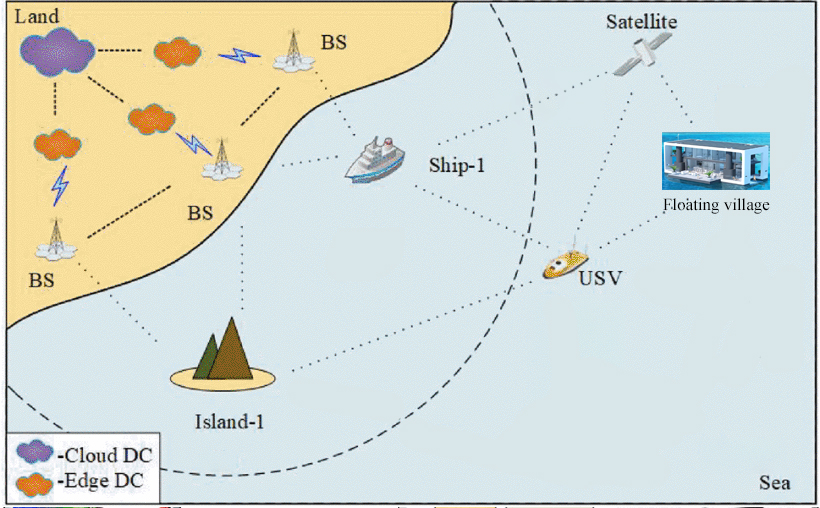
\includegraphics[width=0.8\textwidth]{Figures/A_novel_platform_of_maritime_communication_network.jpg}
\caption{\label{A_novel_platform_of_maritime_communication_network}A novel platform of maritime communication network, Source: \cite{10.1109/ISPA-BDCloud-SocialCom-SustainCom51426.2020.00190}.}
\end{figure}


\subsubsection{Cooperation with network operators}
\label{sec:org9ae04a1}
China Mobile Communications Group Co.,Ltd. (CMCC) is the world's leading communications company. The company can build communication lines, communication base stations and provide long-term maintenance.

\subsubsection{Running cost analysis}
\label{sec:orge9f8aa9}
Generally speaking, the cost of 5G Acer station is composed of main equipment, power supporting equipment and facilities and civil construction (shown in Tables \ref{MainEquipment}, \ref{PowerSupportingEquipmentAndFacilities}, \ref{CivilConstruction}).

\begin{table}[H]
\caption{\label{MainEquipment}Running cost for Main equipment}
\centering
\begin{tabular}{lrll}
\toprule
Name & Quantity & Cost per piece(\pounds) & Total(\pounds)\\
\midrule
BBU & 1.0 & 2,891 & 2,891\\
AAU & 3.0 & 3,012 & 9,036\\
transmission equipment & 1.0 & 6,024 & 6,024\\
\midrule
Total(\pounds) &  &  & 17,951\\
\bottomrule
\end{tabular}
\end{table}

\begin{table}[H]
\caption{\label{PowerSupportingEquipmentAndFacilities}Running cost for Power supporting equipment and facilities}
\centering
\begin{tabular}{lrll}
\toprule
Name & Quantity & Cost per Piece (\pounds) & Total (\pounds)\\
\midrule
Power Supply & 1.0 & 12,048 & 12,048\\
Battery & 4.0 & 1,204 & 4,816\\
air conditioner & 1.0 & 230 & 230\\
Condition monitoring & 5.0 & 1,445 & 7,225\\
\midrule
Total(\pounds) &  &  & 24,319\\
\bottomrule
\end{tabular}
\end{table}

\begin{table}[H]
\caption{\label{CivilConstruction}Running cost for Civil construction}
\centering
\begin{tabular}{lrll}
\toprule
Name & Number & Cost per piece (\pounds) & Total(\pounds)\\
\midrule
computer room & 1 & 610 & 610\\
Ground tower(approx 20m) & 1 & 8,235 & 8,235\\
Labor cost & 1 & 18,072 & 18,072\\
rent (per month) & 1 & 6,097 & 6,097\\
\midrule
Total (\pounds) &  &  & 33,014\\
\midrule
USV rental fee & 1 & 9,638 & 9,638\\
\bottomrule
\end{tabular}
\end{table}

\subsection{Physical Connection}
\label{sec:org83d5ee9}
The real connection between the mainland and the floating village is also indispensable. The floating village needs to provide a safe, reliable, effective connecting method to receive visitors and transport. There are two main parts of the connection. The first one is the dock. The second one is about transportation.

\subsubsection{Dock}
\label{sec:orgab611f0}
In order to clarify the advantages of the aluminium alloy to build the dock, there are some physics properties about aluminium alloy and conventional steel. According to the most used material in the construction, \texttt{Q235} was chosen as the steel in the comparison. Also, except the \texttt{Al-Mg} aluminium alloy, the \texttt{6061-T6} aluminium alloy as the used material for the project whose properties are shown in the  \ref{Physics_Properties_of_aluminium_alloy_and_steel}.

\begin{table}[H]
\caption{\label{Physics_Properties_of_aluminium_alloy_and_steel}Physics Properties of aluminium alloy and steel \cite{10.2749/101686606778995119}}
\centering
\begin{tabular}{llrr}
\toprule
Physical Properties & aluminium alloy & 6061-T6 & Q235\\
\midrule
Limiting Yield Value \(fy /(N\times mm^{-2} )\) & ALMg4.5Mn 140 & 241.4 & 235\\
 & AlMgSi 260 &  & \\
 & AlSnMg 360 &  & \\
\midrule
Ultimate Strength \(fu/(N\times mm^{-2} )\) & ALMg4.5Mn 280 & 289.6 & 375 \textasciitilde{} 460\\
 & AlMgSi 320 &  & \\
 & AlSnMg 410 &  & \\
\midrule
Elastic Modulus E/() & 70.0 & 70.0 & 206.0\\
\(\epsilon_T/\%\) & 10-25 & 10 - 25 & 25 - 30\\
\(\Gamma /(N\times mm^{-2})\) & 26.5 & 27.0 & 78.5\\
\(a/10^{-50}C^{-1}\) & 2.0 & 2.0 & 1.0\\
\bottomrule
\end{tabular}
\end{table}


What can be concluded from the table above is that the \texttt{6061-T1} is the appropriate material for building the dock. The reason is that the physics properties of it shows it is a stable and firm material against the water flush and any other strength challenge such as wind or ocean waves.

The constructing structures are shown in \ref{constructing_structure1} and \ref{constructing_structure2}. After testing the structure, the results are that its limiting load can reach \texttt{1441.22 KN} and the finite element analysis reaches \texttt{1370.05 KN} \cite{10.1061/(ASCE)0887-3828(2001)15:2(68)}.

\begin{figure}[H]
\centering
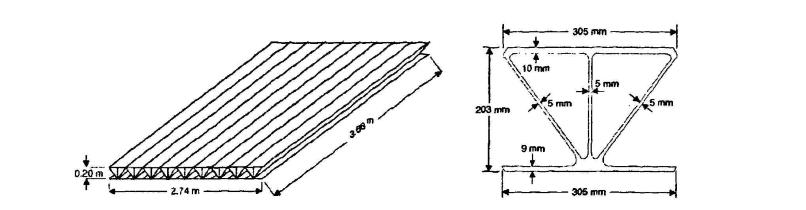
\includegraphics[width=0.8\textwidth]{Figures/constructing_structure1.jpg}
\caption{\label{constructing_structure1}The structure of the dock and its intersecting surface}
\end{figure}

\begin{figure}[H]
\centering
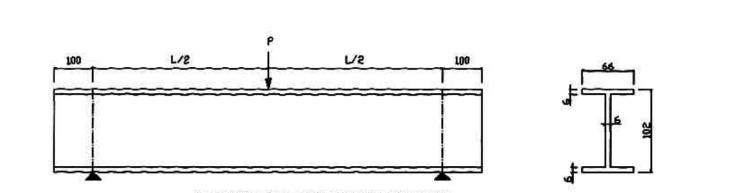
\includegraphics[width=0.8\textwidth]{Figures/constructing_structure2.jpg}
\caption{\label{constructing_structure2}The edge structure of the dock and its intersecting surface}
\end{figure}

Although the cost of building the aluminium alloy dock is more than conventional steel structure, considering the corrosion resistance, the steel dock will cost lots of money to maintain and repair. In the long run, conventional steel structures will cost more than aluminium alloy dock.

\begin{table}[H]
\caption{\label{The_loading_capacity_compare_with_the_same_structure}The loading capacity compare with the same structure \cite{10.2749/101686606778995164}}
\centering
\begin{tabular}{lrrrrr}
\toprule
Material & Mass (kg) & Yield (MPa) & Ultimate Bearing & Weight-strength & Weight-ultimate Bearing\\
 &  &  & Capacity (KN) & Ratio & Capacity Ratio\\
\midrule
6061-T6 & 7.193 & 235.5 & 12.711 & 32.74 & 1.767\\
6061-T6 & 20.912 & 235.0 & 22.467 & 11.238 & 1.074\\
\bottomrule
\end{tabular}
\end{table}

From Figure \ref{The_loading_capacity_compare_with_the_same_structure}, the \texttt{6061-T6} has obviously better weight-strength ratio and weight-ultimate bearing capacity  ratio which means if using the same mass \texttt{6061-T6} with \texttt{Q235}, the \texttt{6061-T6} will support around \texttt{3} times capacity.

\subsubsection{The transporting ships}
\label{sec:org7c6f437}
Different ship types have different functions according to the type of cargo:

\begin{itemize}
\item \textbf{Full passenger ship:} passengers only.
\item \textbf{Passenger and cargo ships:} mainly transporting passengers, supplemented by goods.
\item \textbf{Cargo and passenger ships:} mainly transporting goods, supplemented by passengers.
\item \textbf{Dry cargo ship:} Specific diversity includes container ships, general cargo ships, bulk cargo ships, timber ships and refrigerated ships.
\item \textbf{Container ship:} transport containers.
\item \textbf{General cargo ship:} it mainly transports bundles, bags, barrels and other general cargo.
\item \textbf{Bulk carrier:} transport bulk cargoes such as grain, ore, coal and chemical fertiliser
\item \textbf{Timber and log ship}
\item \textbf{Refrigerated ship:} transporting fish, meat, fruits, vegetables, etc.
\end{itemize}

\section{Business case}
\label{sec:org4605b2e}
\subsection{Budget}
\label{sec:orgf6e1afd}
The table below shows the cost estimates of certain portions of the project. The costs are assumptions made based on actual price of equipment and the budget  list of high-end hotels.

\begin{table}[H]
\caption{\label{TotalCost}The cost of materials and equipment for building floating village}
\centering
\begin{tabular}{rlrll}
\toprule
 &  & \textbf{Quantity} & \textbf{Cost per Unit} & \textbf{Total}\\
\midrule
1 & \textbf{Transportation} &  &  & £24,200\\
\midrule
 & Helicopter & 1 & £10,000 & £10,000\\
 & Boats & 3 & £3,000 & £9,000\\
 & Floating bridge & 2 km & £2,600 & £5,200\\
\midrule
2 & \textbf{Architecture} &  &  & £3,225,300\\
\midrule
 & Electrical equipment & 1 & £1,400,000 & £1,400,000\\
 & Building subject & 1 & £900,000 & £900,000\\
 & Landscape engineering & 1 & £70,000 & £70,000\\
 & Interior decoration & 1 & £650,000 & £650,000\\
 & BioRock System & 1 & £5,300 & £5,300\\
 & Reserved fee & 1 & £200,000 & £200,000\\
\midrule
3 & \textbf{Anti-Roll U Tank System} &  &  & £356,480\\
\midrule
 & Control valve & 12 & £390 & £4,680\\
 & Piping & 6 & £100 & £600\\
 & Control system & 1 & £100,000 & £100,000\\
 & Pump & 2 & £25,000 & £50,000\\
 & Enclosure & 1 & £50,000 & £50,000\\
 & Level sensor & 4 & £300 & £1,200\\
 & Installation fee & 1 & £150,000 & £150,000\\
\midrule
4 & \textbf{Communication equipment} &  &  & £51,115\\
\midrule
 & BBU & 1 & £2,891 & £2,891\\
 & AAU & 3 & £3,012 & £9,036\\
 & Transmission equipment & 1 & £6,024 & £6,024\\
 & Power Supply & 1 & £12,048 & £12,048\\
 & Battery & 4 & £1,204 & £4,816\\
 & Air conditioner & 1 & £230 & £230\\
 & Condition monitoring & 5 & £1,445 & £7,225\\
 & Computer room & 1 & £610 & £610\\
 & Ground tower(approx 20m) & 1 & £8,235 & £8,235\\
\midrule
Total Cost &  &  &  & £3,657,095\\
\bottomrule
\end{tabular}
\end{table}

\subsection{Yearly costs}
\label{sec:org2e8623f}
The following are the maintenance costs required for the hotel over the course of a year of operation (all figures are assumed to be realistic). The floating village hotel has \texttt{20} employees and \texttt{20} rooms, and each room costs \texttt{£500} on average.

\begin{table}[H]
\caption{\label{YearlyCost}The annual expenses required by the floating village in all aspects}
\centering
\begin{tabular}{lrll}
\toprule
Part & Number & Cost per piece & Total\\
\midrule
Platform maintenance cost & 1 & £15,000 & £15,000\\
Maintenance of electrical equipment & 1 & £14,000 & £14,000\\
Average employee salary & 20 & £30,000 & £600,000\\
Storage Cost & 1,500 kWh & £106 & £159,000\\
generating power & 260,000 kWh & £0.09 & £23,400\\
Advertising expenses & 1 & £35,000 & £35,000\\
USV rental & 1 & £9,638 & £9,638\\
Consumption of material & 1 & £5,000 & £5,000\\
\midrule
Yearly cost &  &  & £861,038\\
\bottomrule
\end{tabular}
\end{table}

\subsection{Payback period}
\label{sec:org751e96c}
Assuming an average room rate of \texttt{£500} for this hotel and a room occupancy rate of \texttt{60\%}, We can calculate the RevPAR (Revenue Per Available Room).

\begin{align}
\label{eqRepvar}
RevPAR &= \pounds500\times 0.60 = \pounds300\\
Room\; revenue\; (annual) &= RevPAR \times  n_{rooms} \times  n_{days}\\
       &=> \pounds300\times 20\times 365 = \pounds2,190,000\\
Annual\;profit &= Room\;revenue\; \text{(annual)} - \text{yearly cost}\\
                &=> \pounds2,190,000 - \pounds1,303,118 = \pounds886,882\\
Payback\; period &= 7,000,000/886,882 = 7.89\; (years)
\end{align}

\subsection{Hotel operating income}
\label{sec:orgd56f8b3}
According to the main and secondary business of the enterprise, the enterprise business income can be divided into main business income and other business income. The income generated by the enterprise's recurrent, main business is the main business income, and the income generated by non-recurrent, part-time business transactions is other business income. Usually, the main business income accounts for a significant proportion of the enterprise's revenue and has a greater impact on the enterprise's operating efficiency. Other operating income, on the other hand, accounts for a smaller proportion of an enterprise's revenue.

Modern hotels are tourism and hospitality facilities that provide accommodation and food as well as a variety of other services. There are many sources of income, but the main focus is on the provision of services, with less non-recurring business. It can be divided into: room income, food and beverage income, recreational income, and the hotel can be divided into a number of items as needed. For example, room income includes room rental income, in-room food and beverage income, laundry income, etc.; food and beverage income can be divided into various food and beverage outlets (such as Chinese restaurants, Western restaurants, bars, cafes, etc.); recreational income can be divided into recreational income according to the type of recreation; merchandise income can be divided into the type of merchandise sold; and so on.

\subsection{Strategies for increasing revenue}
\label{sec:orgc48bca1}
\subsubsection{Create brand value}
\label{sec:orgbb85efe}
At a time when hotels are a mature industry and their functional characteristics are not significantly differentiated, it can be crucial for a hotel brand to establish a set of promises to hotel guests and reflect their desires through its brand personality \cite{10.1177/1356766713481218}. Brand personality traits such as sincerity, excitement, competence, sophistication and sturdiness enable consumers to express themselves through the use of the brand \cite{10.1177/1356766713481218}. By creating a good hotel brand name and a slogan can leave a deep impression on customers, and then through a series of marketing means to make the brand image popular.

\subsubsection{Marketing}
\label{sec:orgebfb765}
Firstly, there is the traditional way of marketing. This includes sales people visiting unfamiliar people or companies or telemarketing to explore the market and find target customers. There is also the use of paper media, TV commercials and flyers to attract a large number of customers. Cooperation with some large travel agencies and government activities to expand the influence is also a marketing tool.

The second is marketing using the influence of the internet. The methods are not limited to developing mobile app/website, inviting social software \emph{netizens} to experience and posting the experience on social media platforms to leverage their influence to attract their followers, extensive online advertising, search engine/link/email marketing.

\subsubsection{Increase other income}
\label{sec:org87eda4d}
Undertake commercial events such as banquets, weddings as well as conferences  to increase revenue. A quality service at a higher price as well as a fully packaged sale of the venue. At the same time, a professional venue can be opened up for some interesting exhibitions. The exhibition will attract people from all walks of life to come and spend money and increase the visibility of the hotel. Peripheral products may be developed to give to guests and sell them on the hotel's mobile app. It is also possible to add to the hotel's consumer offerings, such as a spa, beauty salon, gym, various restaurants, etc.

\section{Environment \& Sustainability}
\label{sec:org12179dd}
\subsection{Introduction}
\label{sec:org81418a0}
This section deals with how to make the village environmentally sustainable. This consideration is important to make because the project itself responds to consequences of human activity so avoiding further damage is practical.

In all the design decisions made in sections of the project, environmental sustainability was heavily weighted criteria amongst other options where possible. In the choice of wind power as an energy source over fossil fuelled generators, avoidance of any floatation technology that will give off vibration that affects marine life, the choice of wood, a biodegradable material as the building material of choice. This is not a complete shift as some conventional fossils like those used in boats/ helicopters, the choice of transport and backup generators, but a significant shift.

Below we cover the specific challenges of waste management, water supply and an overall estimated environmental impact of project technologies.

\subsection{Waste-water}
\label{sec:orgbc2375f}
Waste-water management is one of the ways building on water differs from land as there is no default method as in a municipal area. This development will have a similar system to that found on houseboats. The indoor plumbing will be as usual with all the waste flowing to a sewage holding tank with a float regulated pump. In this set up, called honey pot, the sewage is ground into a slurry and pumped to the municipal sewer system via a flexible hose. Since this will be implemented farther out to sea than a houseboat, weighted, flexible marine grade conduits to the land will house the sewage line and appropriate connections to municipal waste systems made.

This setup is chosen because our hotel is a small-scale enterprise. Because the stable method of matter supply is via a direct connection to the mainland, a similar method for wastewater becomes more practical than a wastewater treatment plant. This is coupled with the cost of a treatment plant and the fact that this method has a lower running cost than storage and periodic evacuation of waste or treatment and evacuation of treated water farther out to sea, makes this option better.

\subsection{Other waste}
\label{sec:org4ca5d03}
Other waste described here includes household and food waste. For this scale of application, as other supplies go to the village via boat, these other wastes may be transported back to the mainland for disposal or recycling

On a larger scale village, where food is being grown, the options of composting, anaerobic digestion to produce biogas for cooking or heating is an option that may be explored

\subsection{Water Supply}
\label{sec:org80b4a77}
Water will be provided to the island via connections to mainland water supply through conduits as in the wastewater section above. In addition, the architecture will allow for gathering rainwater, which will be filtered and added to the supply. These methods ensure cost effectiveness and stability of supply when put together when contrasted with a costly desalination plant that is not appropriate for a project of this scale.

When the village is scaled up to include more platforms and should a village need to be located farther out, a water desalination plant will become a more cost-effective option for both stability of supply and sustainability of the village.

\subsection{Overall Environmental Impact}
\label{sec:org7552295}
As a measure of the impact of specific human activities or projects to the environment, indicators are checked and assessments to determine areas of interest carried out. While this is done quantitatively in industry in terms of relevant quantities, only the potential for these impacts will be assessed on a 5-point scale for this report. A breakdown of indicators to be regularly checked during the lifetime of the project to measure pollution issues and natural resources/assets will also be itemized.

\begin{figure}[H]
\centering
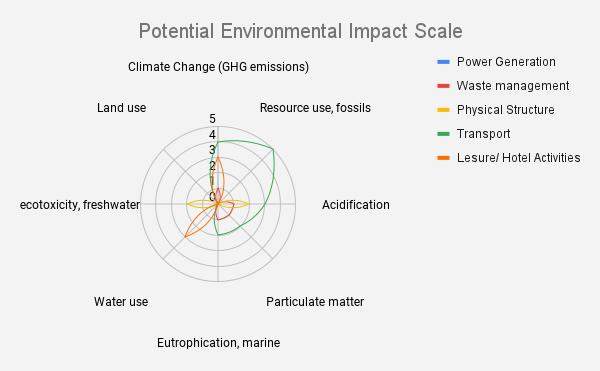
\includegraphics[width=0.8\textwidth]{Figures/PotentialEnvironmentalImpactScale.png}
\caption{\label{PotentialEnvironmentalImpactScale}Potential Environmental Impact Scale}
\end{figure}

The Figure \ref{PotentialEnvironmentalImpactScale}  shows potential impacts to the environment for some sections of the project. The potential impacts considered are global warming, resource use, acidification. As seen above and mentioned in the introduction, because of the technology choices made and because this scale accounts for the period the project runs and not the entire life-cycle, the impact is expected to be low on all aspects except transportation.

During the useful life of the project, some key indicators to be constantly measured as prescribed by OECD \cite{oecdKeyIndicators} are ‘indices of GHG emissions, ozone depletion substances, \texttt{SOx} and \texttt{NOx} emission intensities, municipal waste generation intensities and waste water treatment connection rates as well as intensity of use of water, forest, fish and energy resources’.

\subsection{Further Recommendations}
\label{sec:org8997c40}
For sustainable food supply when there are more platforms, Hydroponics, aquaponics maybe employed to provide food for the village possibly using waste heat from desalination process or heat from waste

\section{Conclusion}
\label{sec:orgf13c939}
As an effective solution to the problem of sea level rise, the report discusses the structural, environmental, transport and cost aspects of sea villages, systematically demonstrating the integrity and feasibility of the project. It discusses viable solutions to different challenges and chooses the best option.

In terms of its structure, it focuses on describing what technology is used to achieve floatation and considers how to achieve the stability of the structure on the sea deciding on Biorock anchors for mooring and an anti-roll tank for stabilization.

Power is to be supplied through offshore wind turbines supplemented by back up diesel generators and battery storage. A rough cost estimate for floating the structure, a communication set up and provision of transport are made and  the assumed investment for the project to about \texttt{£7} million has an expected payback period of \texttt{7.89} years.

The means of transport to the mainland is designated via ships and boats with a floating dock attached to the village platform and 5G networks are to be deployed for communication with the mainland. From an environmental standpoint, it determines that connections to the mainland for waste management and water supply is the best method for stability as well as prescribing environment indicators to monitor the state of the surrounding sea.

\section{Bibliography}
\label{sec:orge305942}
\bibliography{biblio}
\bibliographystyle{IEEEtran}
\end{document}
